% !TeX root = ../../../../thesis.tex

\subsection{Testbed}
	\label{subsec:dc-testbed}

	To be able to test all aspects of the system a testbed was created.
	This testbed will allow the testing of the correlation calculations as discussed in \autoref{sec:mapping-problem}, the interference solutions (\autoref{subsec:continuous-method-modulation}), and the performance of the modulator and current-sampler.


	\begin{figure}[ht]
		\centering
		\includegraphics[angle=0,width=0.6\textwidth,height=.9\textheight,keepaspectratio]{chapters/hardware-chapters/DC/dc-test-bed/dc-test-bed-picture.JPG}
		\caption{Picture of the DC testbed, showing the six LED strips, current sources, current sampler and an Arduino board.}
		\label{fig:dc-test-bed-picture}
	\end{figure}

	\begin{figure}[ht]
		\centering
		\includegraphics[angle=0,width=1.0\textwidth,keepaspectratio]{chapters/hardware-chapters/DC/dc-test-bed/dc-test-bed-architectural.JPG}
		\caption{Architectural overview of the DC testbed. Six LED modulators are connected in parallel with each other and in series with the current sampler.}
		\label{fig:dc-test-bed-architectural}
	\end{figure}


	The testbed works with a DC power supply and has six individual controllable current sources.
	Each current source powers one LED fixture.
	The testbed itself can be seen in \autoref{fig:dc-test-bed-picture} and an architectural overview of how everything is connected to each other can be seen in \autoref{fig:dc-test-bed-architectural}.


	The aim of the testbed was to use commercial LEDs. 
	The LED fixtures used in this testbed all came from the same commercial LED, which can be found in \cite{commercial-230v-ac-led-aliexpress}.
	A picture of the LED can be seen in \autoref{fig:ac-commercial-230v-ac-led}.
	The strips are taken out of this commercial LED and used individually for this testbed.


	The current is measured by a series resistor and fed to the ADC of a micro-controller.
	The entire schematic of the DC testbed can be found in \autoref{app:dc-test-bed}. 

	The current sources and therefore the LEDs, can be toggled on and off by a micro-controller.
	By toggling the current sources on and off, the current that flows through the series resistor will change accordingly.
	A change of voltage over the series resistor can then be measured by the ADC.

	The measured current from the DC testbed can be seen in \autoref{fig:raw-dc-test-bed-data-short}.
	In this experiment, all six LEDs are modulating with the unique ID that was assigned to each LED.
	The voltage drop over the resistor is measured with the ADC.
	The raw ADC value can be seen on the left y-axis and the calculated aggregated current that is drawn can be seen on the right y-axis.
	From this figure seven distinguishable states can be seen.
	When there are no LEDs on, all LEDs are encoding a `0' data bit, the current is zero.
	When one of the six LEDs is transmitting a `1' data bit, the current jumps to roughly 50 mA.
	When two of the six LEDs are encoding a `1', the current is roughly 100 mA and so on.


	\begin{figure}
		\centering
		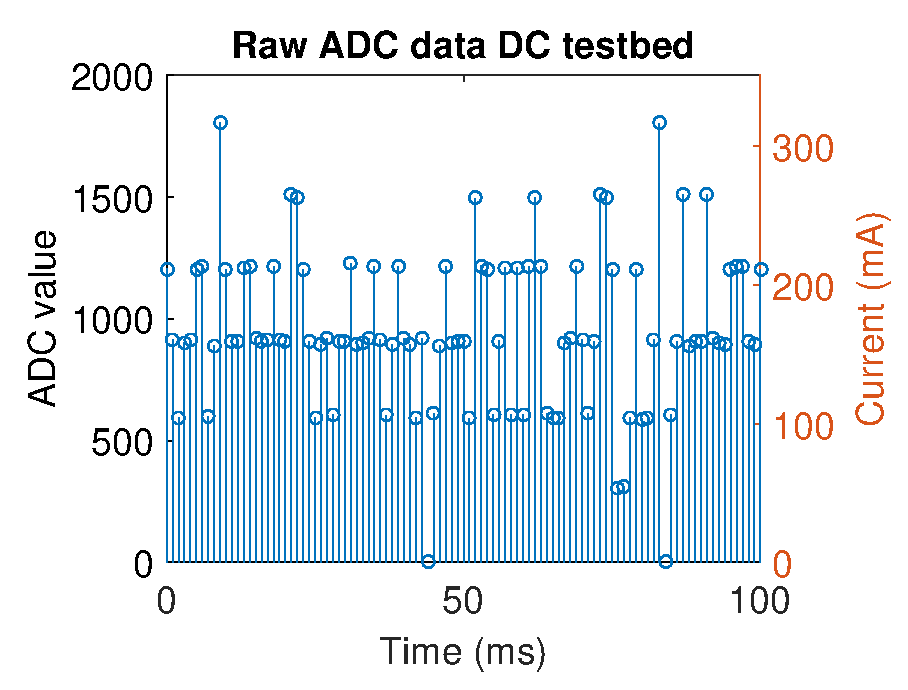
\includegraphics[angle=0,width=0.7\textwidth,keepaspectratio]{chapters/hardware-chapters/DC/dc-test-bed/dc-test-bed-raw-data.eps}
		\caption{Raw current data from the DC testbed with the six LEDs modulating with their unique IDs.}
		\label{fig:raw-dc-test-bed-data-short}
	\end{figure}



	An evaluation of this testbed is done in \autoref{subsec:dc-testbed-eval} where a longer signal will be shown along with correlation data to identify if a certain LED is on, while the other LEDs are modulating and thereby causing interference.










